\documentclass{sintefbeamer}

% meta-data
\title{数据结构与算法\\ Data Structure and Algorithm}
\subtitle{Introduction}
\author{\href{mailto:zlp@upc.edu.cn}{ZHANG Luping}}
\date{\today}
\titlebackground{images/background}

% document body
\begin{document}

\maketitle

\section{课程介绍}
\begin{frame}{课程所处地位}


  \begin{itemize}
    \item \textbf{《数据结构与算法》}是信息管理专业的\textcolor{red}{核心基础课程}之一。
    \item 它为学生提供解决实际问题和优化信息系统的\textcolor{red}{关键工具和技术}。
    \item 该课程与其他信息管理科学相关课程(如《管理信息系统》、《面向对象程序设计》、《商务智能与数据挖掘》、《信息系统分析与设计》等)相互关联,\textcolor{red}{构建了信息管理专业的技术基础}。
  \end{itemize}
  \begin{figure}
    \centering
    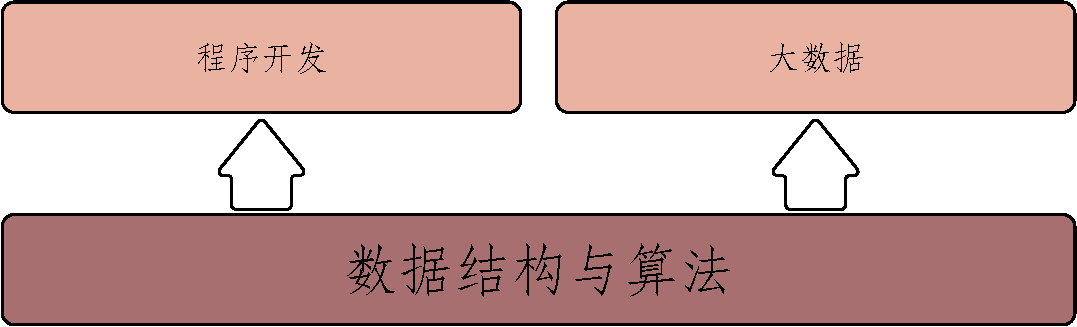
\includegraphics[width = 0.5\textwidth]{./images/import.pdf}
  \end{figure}


\end{frame}

\begin{frame}
  \frametitle{课程特征}

  \begin{itemize}
    \item \textbf{抽象性强}:数据结构与算法课程涉及到抽象的数据模型和算法设计,需要学生具备抽象思维和逻辑推理能力。
    \item \textbf{实践性强}:该课程注重实践操作和算法实现,学生需要通过编程实践来加深对数据结构和算法的理解和应用。
    \item \textbf{算法思维培养}:该课程强调培养学生的算法思维,即解决问题的思考方式和技巧,让学生具备分析、设计和优化算法的能力。
  \end{itemize}

\end{frame}

\begin{frame}
  \frametitle{主要讲授内容}

  \begin{itemize}
    \item 基本数据结构:包括数组、链表、栈、队列、树等常用数据结构的定义、实现和操作。
    \item 常用算法:涵盖排序算法、搜索算法、图算法等,如冒泡排序、快速排序、二分查找、广度优先搜索、最短路径算法等。
    \item 数据结构和算法的应用:介绍数据结构和算法在实际问题求解和信息管理系统中的应用,如数据库、大数据分析等领域。
  \end{itemize}

\end{frame}


\section{目标}

\begin{frame}
  \frametitle{期望目标}

  \begin{enumerate}
    \item 熟悉常见的数据集合抽象(例如栈、队列、列表、树、映射)。
    \item 理解实现常见数据结构的高效算法策略。
    \item 能够从理论和实验的角度分析算法性能,并识别不同策略之间的常见权衡和取舍。
    \item 能够基于Python语言明智地使用现有的数据结构和算法。
    \item 能够应用数据结构和算法解决复杂问题。
  \end{enumerate}

\end{frame}

\section{算法概述}

\begin{frame}{Declarative knowledge vs. Imperative knowledge}

  All knowledge can be thought of as either \textcolor{red}{\textbf{declarative (陈述性的)or imperative (命令性的)}}.

  \begin{itemize}[<+->]
    \item \textcolor{red}{\textbf{Declarative knowledge}} is composed of statements of fact.
          \begin{itemize}
            \item \textit{The square root of $x$ is a number $y$ such that $y \times y = x$},
            \item \textit{It is possible to travel by train from Qingdao to Beijing}
          \end{itemize}
    \item \textcolor{red}{\textbf{Imperative knowledge}} is ``how to'' knowledge, or recipes for deducing information.
  \end{itemize}

\end{frame}

\begin{frame}
  \frametitle{A way to compute the square root of a number}

  \pause

  \begin{enumerate}
    \item Start with a guess, $g$.
    \item If $g \times g$ is close enough to $x$, stop and say that $g$ is the answer.
    \item Otherwise, create a new guess by averaging $g$ and $\frac{x}{g}$, i.e., $\frac{(g + \frac{x}{g})}{2}$.
    \item Using this new guess, which we again call $g$, repeat the process until $g \times g$ is close enough to $x$.
  \end{enumerate}

\end{frame}

\begin{frame}
  \frametitle{Definition of \textcolor{red}{algorithm}}

  \begin{itemize}[<+->]
    \item Note that the description of the method is \textbf{a sequence of simple steps, together with a flow of control} that specifies when to execute each step. Such a description is called an \textcolor{red}{\textbf{algorithm}}.\\[5pt]
    \item More formally, \textit{an algorithm is \textcolor{blue}{a finite list of instructions} describing a set of \textbf{computations} that when executed on \textcolor{blue}{a set of inputs} will proceed through a sequence of well-defined states and eventually produce \textcolor{blue}{an output}}.
  \end{itemize}

\end{frame}

\begin{frame}[fragile]{Examples: Perfect cube root}
  This code prints the integer cube root, if it exists, of an integer. If the input is not a perfect cube, it prints a message to that effect.

  \begin{block}{}
    \begin{lstlisting}[language=Python]
      # Find the cube root of a perfect cube
      x = int(input("Enter an integer: "))
      ans = 0
      while ans**3 < abs(x):
          ans += 1
      if ans**3 != abs(x):
          print(x, "is not a perfect cube")
      else:
          if x < 0:
              ans = -ans
          print("Cube root of”, x, "is", ans)
    \end{lstlisting}
  \end{block}
\end{frame}

\begin{frame}[fragile]{Examples: Prime number}
  This code tests whether an integer is a prime number and returning the smallest divisor if it is not.
  \pause
  \begin{block}{}
    \begin{lstlisting}[language=Python]
      # Test if an int > 2 is prime. If not, print smallest divisor
      x = int(input("Enter an integer greater than 2: "))
      smallest_divisor = None
      for guess in range(2, x):
          if x%guess == 0:
              smallest_divisor = guess
              break
      if smallest_divisor != None:
          print("Smallest divisor of", x, "is", smallest_divisor)
      else:
          print(x, "is a prime number")
    \end{lstlisting}
  \end{block}
\end{frame}

\begin{frame}[fragile]{Examples: \textcolor{airforceblue}{Finger exercise}}
  Change the code in previous slide so that it returns the largest rather than the smallest divisor. \\[10pt]

  \pause
  Hint: if $y \times z = x$ and $y$ is the smallest divisor of $x$, $z$ is the largest divisor of $x$.
\end{frame}

\begin{frame}[fragile]
  \frametitle{Examples: Approximation to the square root of $x$}

  \begin{block}{}
    \begin{lstlisting}[language=Python]
      epsilon = 0.01
      step = epsilon**2
      num_guesses = 0
      while abs(ans**2 - x) >= epsilon and ans <= x:
          ans += step
          num_guesses += 1
      print("number of guesses = ', num_guesses)
      if abs(ans**2 - x) >= epsilon:
          print("Failed on square root of", x)
      else:
          print(ans, "is close to square root of", x)
    \end{lstlisting}
  \end{block}

\end{frame}

\section{数据结构概述}

\section{参考书目}

\backmatter

\end{document}
